
\section{Introduction}


\subsection{Motivation}
% Choice overload
% Aktuelle Situation in der Kleidungsbranche
% kurzer Einblick in Recommender systems (wird spaeter weiter ausgefuehrt)
When a typical customer enters a shop or department store, he often gets confronted with a very large amount of products he can choose from.
This is especially true, when searching for products online on a web shop.
The commonly well-known web shop \gls{amazon.com} for instance, provides about 280 million different products on their internet presence solely for the United States - there are even more products offered world wide.\citep{marketplaceanalytics:2014}
Even shops dedicated to only a special kind of product can have a wide array of products.
On \gls{zalando}, a German online shop dedicated to clothing, one can choose out of 150.000 products and 1.500 different brands.\citep{visser:2014}\\

%\paragraph{Choice Overload}
\index{Choice Overload}
There is a general belief that great choice pleases the customers needs.
However it is actually proven, that this idea is not fully correct and reality is much more complex.
Already in 2000 a group of scientists demonstrated that a great variety can also have negative effects.
It is proven, that large assortments can lower the customers willingness to purchase products.\citep[p.~312-313]{diehl:2010}
Furthermore to much choice can also lower the customers satisfaction.\citep[p.~320]{diehl:2010}
The state of beeing confronted with an overwhelming range of choice and therefore having trouble finding the right product is commonly known as choice overload.\citep[p.~454]{stanton:2012}
Even though huge sortiments of products attract user, because the generally like to have the possibility to choose, it increases the psychological costs to filter out relevant products and make a decision.
In the end the whole benefit the user may get from a huge assortment of products gets fully consumed by the energy the user has to spend in order to find a good that meets his expectations.
\citep[p.~64]{bollen:2010}

\index{Recommender System}
One possible solution to solve problems caused by choice overload are recommender systems (RS) as they help users finding relevant items they like, by guiding him to those items in a huge space of products.\citep[p.~63]{bollen:2010}
Since especially online-shops have a overwhelming assortment of products, they struggle most with the problem of overloading their potential customers with choices.
Therefore many \gls{e-commerce} sites have already implemented recommendation systems (RS) to aid their customers by finding the right product.
Popular e-commerce sites such as Amazon.com and \gls{eBay} rely on RS in order to satisfy their customers needs.
In fact some vendors even use multiple RS for different use cases to maximise the support they can provide to customers.
\citep[p.~158]{schafer:1999}
There are different possible approaches to recommendation systems and some of them will be discussed in the later sections (section~\ref{sec:recommenderapproaches}) of this thesis.
This thesis however focuses on implementing a recommender system, all necessary steps towards it and the evaluation of its aptitude.
As algorithm for the recommender engine Rocchio's algorithm will be implemented.
Also there will be some alternative ways of input data collection regarding the users preferences.


\subsection{Research question}
{\color{red} Forschungsfragen}
When designing a recommendation system there are some questions, such as the requirements to a recommender system, left to solve.
In the following requirements on a recommender system will be defined.\\
The basic structure of this thesis will orient itself on the research questions.\\
At first the general fundamentals of RS will be explained.
Since a major goal of this thesis is the implementation of an RS it is necessary to identify the core components of which a RS is build of and the tasks it has to solve.\\



\begin{figure}[h]
    \center
    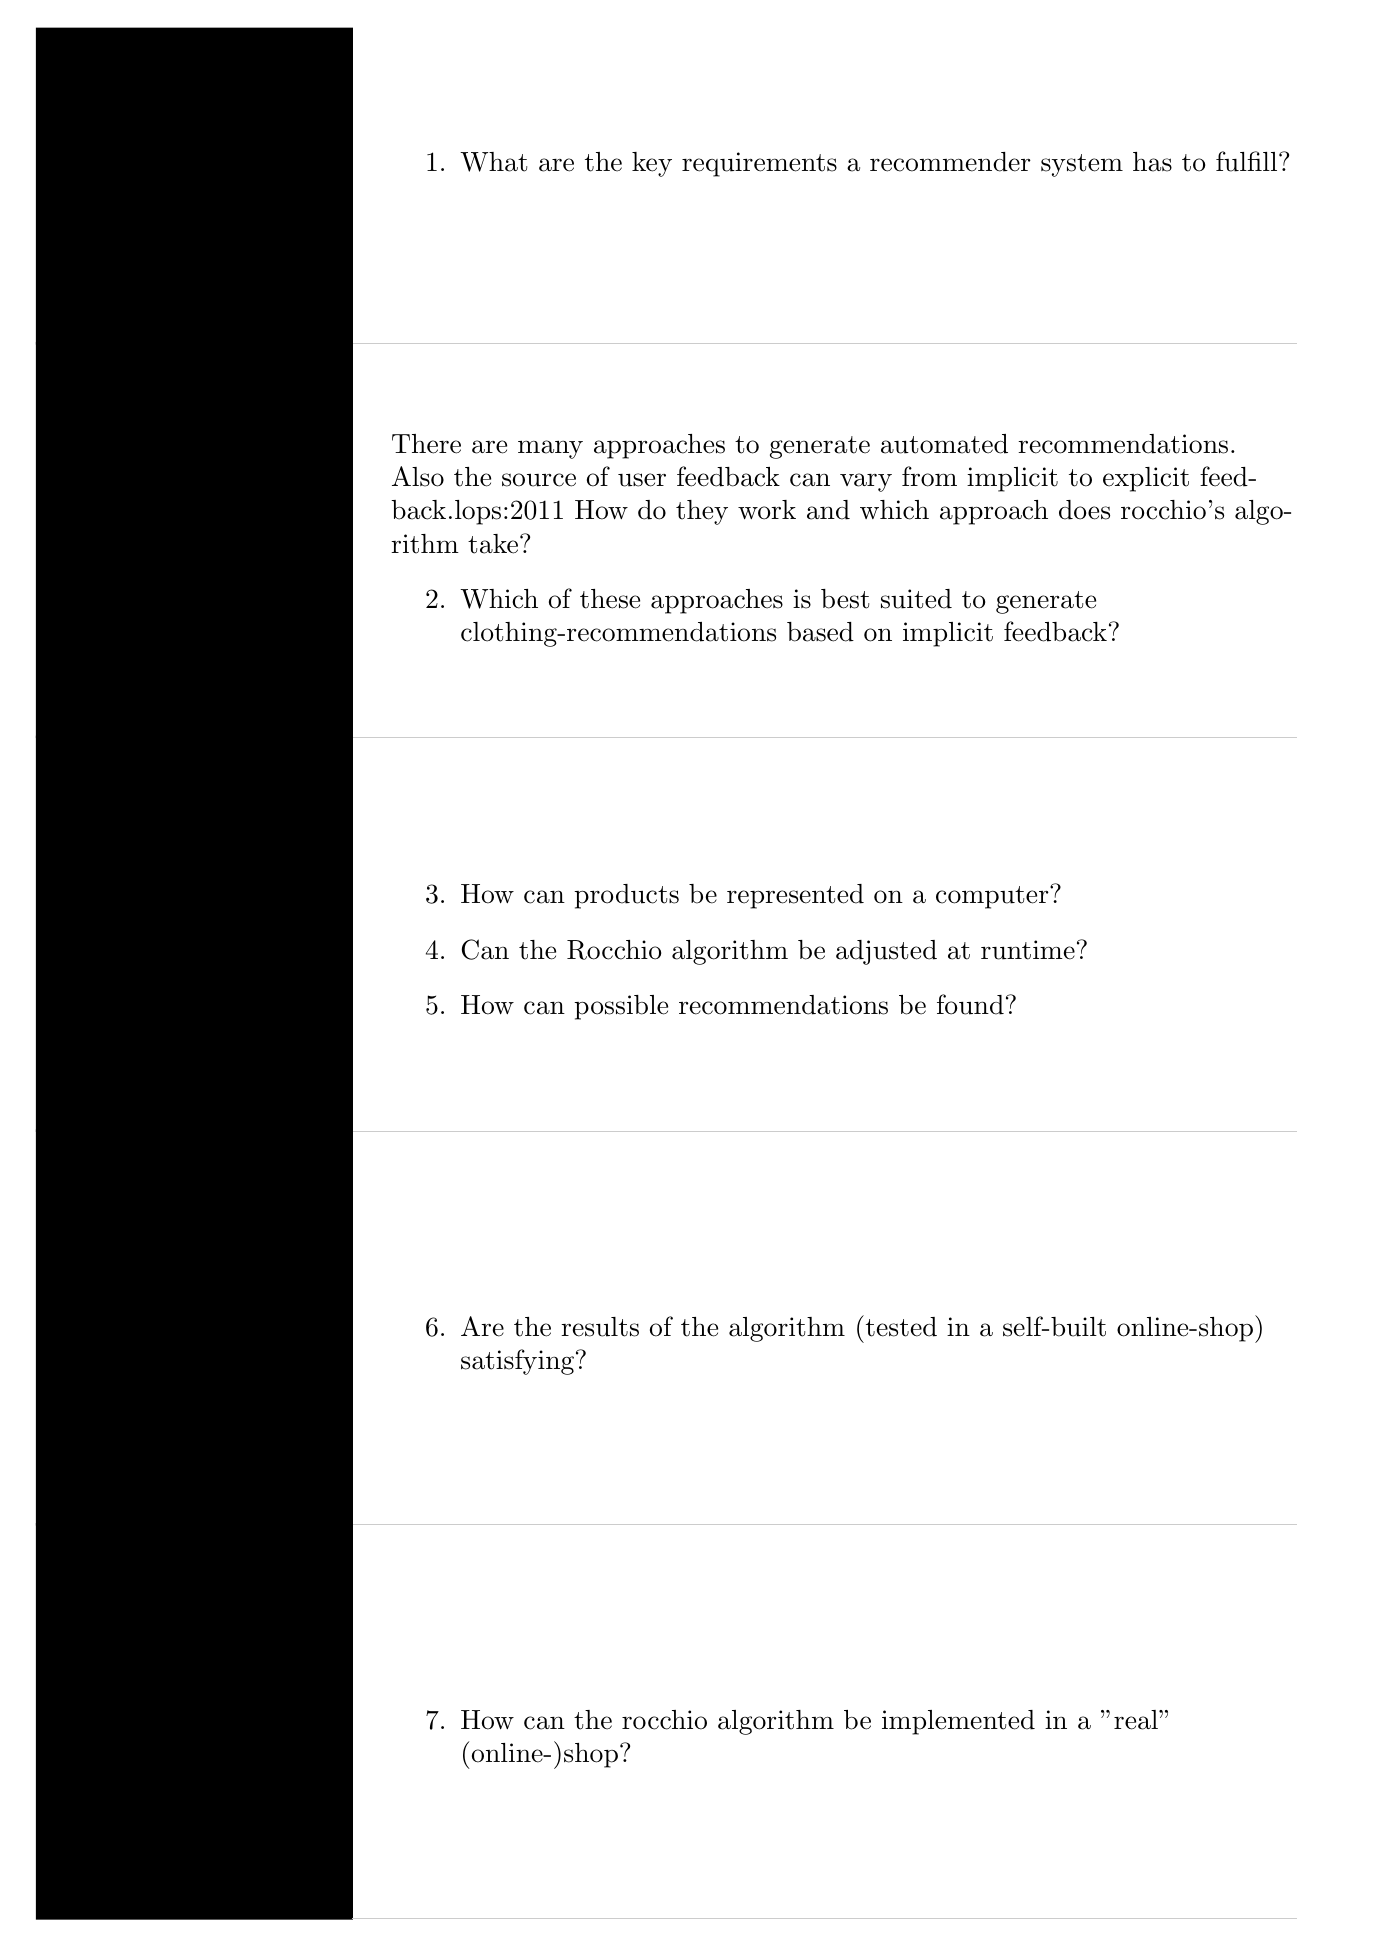
\begin{tikzpicture}
        \def\dustTempLineWidth{12cm}
        \def\dustTempNodeWidth{4cm}
        \def\dustTempNodeHeight{4cm}
        \def\dustTempArrowHeight{1cm}
        \def\dustTempYShift{0cm}

        \def\dustTempYShift{0 * -1 * (\dustTempNodeHeight + \dustTempArrowHeight)}
        \draw[thick,fill=\dustRowFirst]
            (0,0)--(\dustTempNodeWidth /2,-1* \dustTempArrowHeight)--(\dustTempNodeWidth,0)--(\dustTempNodeWidth,\dustTempNodeHeight)--(0,\dustTempNodeHeight)--cycle;
        \node[text width=\dustTempNodeWidth,text centered,yshift=\dustTempYShift] at (\dustTempNodeWidth /2,\dustTempNodeHeight /2)
        {
            \textbf{requirements on a recommender system}
        };
        \node[text width=\dustTempLineWidth,align=left,yshift=\dustTempYShift] at ({\dustTempNodeWidth + \dustTempLineWidth /2 + 0.5cm},\dustTempNodeHeight/2 + \dustTempArrowHeight /2) {
            \begin{enumerate}
                \item What are the key requirements a recommender system has to fulfill?
            \end{enumerate}
        };
        \draw[thin,Black!20,yshift=\dustTempYShift] (\dustTempNodeWidth,0)--(\dustTempNodeWidth + \dustTempLineWidth,0);

        \def\dustTempYShift{1 * -1 * (\dustTempNodeHeight + \dustTempArrowHeight)}
        \draw[thick,fill=\dustRowSecond,yshift=\dustTempYShift]
            (0,0)--(\dustTempNodeWidth /2,-1 * \dustTempArrowHeight)--(\dustTempNodeWidth,0)--(\dustTempNodeWidth,\dustTempNodeHeight+\dustTempArrowHeight)--(\dustTempNodeWidth /2,\dustTempNodeHeight)--(0,\dustTempNodeHeight + \dustTempArrowHeight)--cycle;
        \node[text width=\dustTempNodeWidth,text centered,yshift=\dustTempYShift] at (\dustTempNodeWidth /2,\dustTempNodeHeight /2)
        {
            \textbf{different approaches}
        };
        \node[text width=\dustTempLineWidth,align=left,yshift=\dustTempYShift] at ({\dustTempNodeWidth + \dustTempLineWidth /2 + 0.5cm},\dustTempNodeHeight /2 + \dustTempArrowHeight /2)
        {
            %\begin{quote}
                There are many approaches to generate automated recommendations. % such as "content-based", "collaborative filtering", "demographic", "knowledge-based", "community-based".\citep[p.~10-12]{ricci:2011}
                Also the source of user feedback can vary from implicit to explicit feedback.\citep[p.~76]{lops:2011}
                How do they work and which approach does rocchio's algorithm take?
            %\end{quote}
            \begin{enumerate}
                \setcounter{enumi}{1}
                \item Which of these approaches is best suited to generate clothing-recommendations based on implicit feedback?
            \end{enumerate}
        };
        \draw[thin,Black!20,yshift=\dustTempYShift] (\dustTempNodeWidth,0)--(\dustTempNodeWidth + \dustTempLineWidth,0);

        \def\dustTempYShift{2 * -1 * (\dustTempNodeHeight + \dustTempArrowHeight)}
        \draw[thick,fill=\dustRowFirst,yshift=\dustTempYShift]
        (0,0)--(\dustTempNodeWidth /2,-1 * \dustTempArrowHeight)--(\dustTempNodeWidth,0)--(\dustTempNodeWidth,\dustTempNodeHeight+\dustTempArrowHeight)--(\dustTempNodeWidth /2,\dustTempNodeHeight)--(0,\dustTempNodeHeight + \dustTempArrowHeight)--cycle;
        \node[text width=\dustTempNodeWidth,text centered,yshift=\dustTempYShift] at (\dustTempNodeWidth /2,\dustTempNodeHeight /2)
        {
            \textbf{computer representation}
        };
        \node[text width=\dustTempLineWidth,align=left,yshift=\dustTempYShift] at ({\dustTempNodeWidth + \dustTempLineWidth /2 + 0.5cm},\dustTempNodeHeight /2 + \dustTempArrowHeight /2)
        {
            \begin{enumerate}
                \setcounter{enumi}{2}
                \item How can products be represented on a computer?
                \item Can the Rocchio algorithm be adjusted at runtime?
                % fuer neue nutzer schnell lernend
                % am anfang einer neuen Mode-Saison schnell lernend
                \item How can possible recommendations be found?
            \end{enumerate}
        };
        \draw[thin,Black!20,yshift=\dustTempYShift] (\dustTempNodeWidth,0)--(\dustTempNodeWidth + \dustTempLineWidth,0);

        \def\dustTempYShift{3 * -1 * (\dustTempNodeHeight + \dustTempArrowHeight)}
        \draw[thick,fill=\dustRowSecond,yshift=\dustTempYShift]
        (0,0)--(\dustTempNodeWidth /2,-1 * \dustTempArrowHeight)--(\dustTempNodeWidth,0)--(\dustTempNodeWidth,\dustTempNodeHeight+\dustTempArrowHeight)--(\dustTempNodeWidth /2,\dustTempNodeHeight)--(0,\dustTempNodeHeight + \dustTempArrowHeight)--cycle;
        \node[text width=\dustTempNodeWidth,text centered,yshift=\dustTempYShift] at (\dustTempNodeWidth /2,\dustTempNodeHeight /2)
        {
            \textbf{testing}
        };
        \node[text width=\dustTempLineWidth,align=left,yshift=\dustTempYShift] at ({\dustTempNodeWidth + \dustTempLineWidth /2 + 0.5cm},\dustTempNodeHeight /2 + \dustTempArrowHeight /2)
        {
            \begin{enumerate}
                \setcounter{enumi}{5}
                \item Are the results of the algorithm (tested in a self-built online-shop) satisfying?
            \end{enumerate}
        };
        \draw[thin,Black!20,yshift=\dustTempYShift] (\dustTempNodeWidth,0)--(\dustTempNodeWidth + \dustTempLineWidth,0);

        \def\dustTempYShift{4 * -1 * (\dustTempNodeHeight + \dustTempArrowHeight)}
        \draw[thick,fill=\dustRowFirst,yshift=\dustTempYShift]
            (0,0)--(\dustTempNodeWidth,0)--(\dustTempNodeWidth,\dustTempNodeHeight + \dustTempArrowHeight)--(\dustTempNodeWidth /2,\dustTempNodeHeight)--(0,\dustTempNodeHeight + \dustTempArrowHeight)--cycle;
        \node[text width=\dustTempNodeWidth,text centered,yshift=\dustTempYShift]at (\dustTempNodeWidth /2,\dustTempNodeHeight /2)
        {
            \textbf{outlook}
        };
        \node[text width=\dustTempLineWidth,align=left,yshift=\dustTempYShift] at ({\dustTempNodeWidth + \dustTempLineWidth /2 + 0.5cm},\dustTempNodeHeight /2 + \dustTempArrowHeight /2)
        {
            \begin{enumerate}
                \setcounter{enumi}{6}
                \item How can the rocchio algorithm be implemented in a "real" (online-)shop?
            \end{enumerate}
        };
        \draw[thin,Black!20,yshift=\dustTempYShift] (\dustTempNodeWidth,0)--(\dustTempNodeWidth + \dustTempLineWidth,0);

    \end{tikzpicture}

    \caption{Research questions}

\end{figure}


%Wie kann ein system konzeptioniert und implementiert zu werden um efektive kleidungsempfehlung basierend auf implizitem feedback zu geben?


%- Forschungsmethodik/Vorgehen
%   -- vorgehen mit beispiel der Forschungsfragen



\subsection{Aufbau}

{\color{red}
    Aufgliederung zwischen recherche von state of the art
    und prototyp/impl.



    Ubersicht ueber die Forschugnsfragen
    verweis auf die relevanten textstellen
    beantwortung der Fragen mit explizitem Bezug darauf

    Umschreibung von sec'information retrieval' (kein grosses fass aufmachen)
    zusamenfassen der kapitel IR und Rocchio (evtl. grosses kapitel rocchio mit hinleitung ueber die vectoren)


    Impl >> design and implementation

    Technical details weg lassen (glossary?)


    conclusion
        -summary
            - limitations
        -outlook
}
